Producing a dataset suitable for analysis involves the workflow specified in \ref{analysis-workflow}. The workflow involves configuration of \textit{nETL} tasks to load data from CSVs into CouchDB, authoring of a CouchDB design doc, including a view function (MapReduce) and a list function, asking CouchDB to build the index, retrieving the indexed result via the list function specified in the design document and working with the joined dataset in Excel.

In terms of defining MapReduce tasks, the map function is always user-defined, whereas a built-in reduce function (\_stats) is always used. The built-in reduce function are implemented within the main Erlang process, which according to the documentation offers a performance boost since the IO transfer cost between the Erlang process and the view engine (couchjs.exe by default) is negated. Working on a Windows machine the IO cost is apparently exaggerated (see the slack correspondence with Jan Lehnardt in appendix \ref{slack-1-nov}) due to the difference between Unix-based and Windows kernel implementations.

Analyses are conducted in an iterative fashion; with each iteration an increasing volume of data is handled so as to gain insight into the viability of handling varying amounts of data in CouchDB. Data volume is controlled by the number of courses analyses (more courses taken into account results in higher volumes of data), And the number of entities joined together (grades \& FU data vs grades, FU data, \& Sakai usage). Results are discussed in terms of the insights into business domain (EDM) as well as the effectiveness of the data-mining approach. Runtime results of \textit{nETL}, CouchDB indexing times, database/index storage footprints are shown in Table \ref{performance-analysis}.

\begin{figure}[ht]
    \centering
    \begin{mdframed}
        \centering
        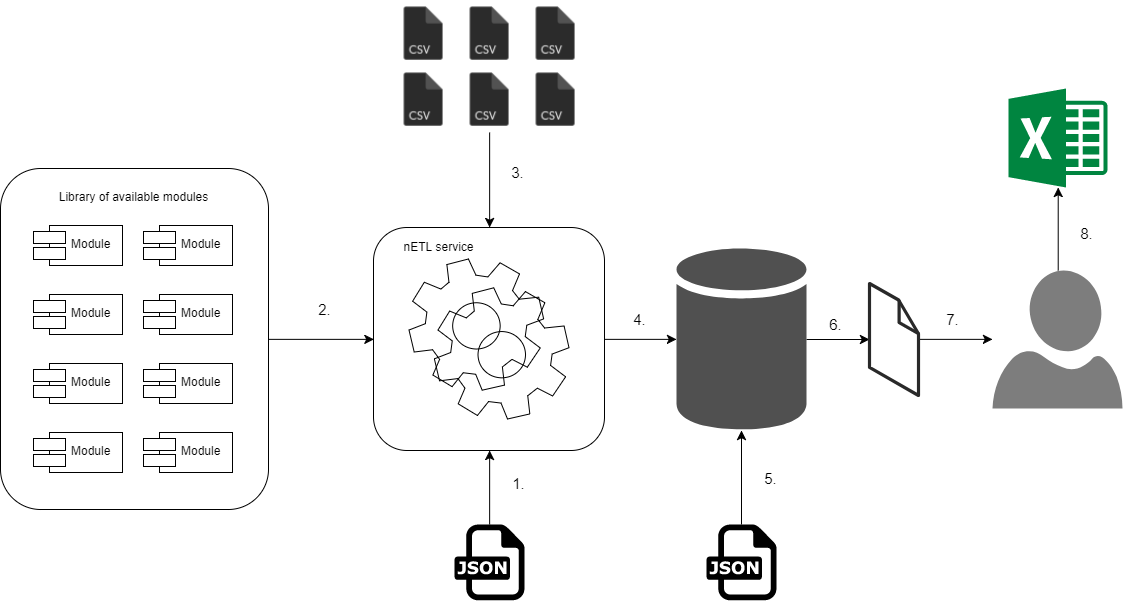
\includegraphics[scale=0.35]{./resources/figures/analysis-workflow.png}
    \end{mdframed}
    \caption[Analysis Workflow]{\textbf{Figure \ref{analysis-workflow}: Workflow to perform an analysis.}1) User creates a configuration file (JSON) that is loaded into the running \textit{\_nETL} service. This configuration includes instructions on which CSVs to load, which modules should be loaded to process the CSVs, and configurations for the modules. 2) Modules are loaded from a library of available modules into the \textit{\_nETL} service. 3) CSVs are loaded into the service, and transformations are applied to the CSV data as specified by the configuration in (1). 4) Data from the CSVs is loaded into CouchDB; this is also achieved via a module specified in (1). 5) A user creates a CouchDB design document, specifying the MapReduce functions, and a List function. 6) The user asks CouchDB to produce the view index as specified by the design document in (5). 7) The user retrieves the data from the view index using the list function specified in (5). 8) The user then loads the resultant CSV into Excel to produce useful metrics.}
    \label{analysis-workflow}
\end{figure}





\begin{table}[h]
    \begin{threeparttable}
        \textbf{Table \ref{performance-analysis}}\par\medskip\par\medskip
        \caption[Software performance analysis]{Running time analysis of \textit{nETL} tasks and CouchDB MapReduce indexing}
        \label{performance-analysis}
        \begin{tabularx}{\textwidth}{>{\hsize=1\hsize}Y>{\hsize=1\hsize}X>{\hsize=1\hsize}X>{\hsize=1\hsize}X>{\hsize=1\hsize}X}
            \toprule
            \mC{c}{}                                               & \mC{c}{Run 1} & \mC{c}{Run 2} & \mC{c}{Run 3} & \mC{c}{Run 4} \\
            \midrule
            Demographic lines extracted                            & 12 219        & 12 219        & 12 219        &               \\
            Demographic lines loaded                               & 1 381         & 9 874         & 595           &               \\
            Demographic task time (sec)\tnote{\textsuperscript{1}} & 2.488         & 3.114         & 6.755         &               \\
            Grade lines extracted                                  & 513 872       & 513 872       & 513 872       &               \\
            Grade lines loaded                                     & 1 891         & 79 849        & 738           &               \\
            Grade task time (sec)\tnote{\textsuperscript{1}}       & 37.684        & 42.001        & 97.221        &               \\
            Events lines extracted                                 & -             & -             & 44 420 508    &               \\
            Events lines loaded                                    & -             & -             & 661 555       &               \\
            Events task time (sec)\tnote{\textsuperscript{1}}      & -             & -             & 2 225.44      &               \\
            CouchDB footprint (MB)\tnote{\textsuperscript{2}}      & 0.9           & 23.2          & 172.1         &               \\
            View calculation time (sec)\tnote{\textsuperscript{3}} & 0.685         & 49.042        & 340.413       &               \\
            View size (MB)                                         & 0.813         & 143           & 521           &               \\
            \bottomrule
        \end{tabularx}
        \scriptsize
        \begin{tablenotes}
            \item[\textsuperscript{1}]Tasks are run asynchronously, so time taken includes processing of other tasks in this run. Task run times are printed out to the log
            \item[\textsuperscript{2}]This is representative of the amount of data processed by \textit{nETL}
            \item[\textsuperscript{3}]CouchDB views are calculated per shard. By default a database contains 8 shards (even in single node mode). The log file shows start and end times of view calculations for each shard, the time is taken as time the first shard starts indexing, to the time the last shard stops indexing.
        \end{tablenotes}
    \end{threeparttable}
\end{table}

todo:

Hi Sonia.

I’m looking at the two approaches to using MapReduce to aggregate data across different entities in CouchDB.

A bit about how view are produced in CouchDB:
CouchDB iterates through the docs, and runs the map function on every document, which the user configures to ‘emit’ values. For my function, the emitted value is a tuple with 11 indexes, with every value initialized at 0. So it’s this: [0,0,0,0,0,0,0,0,0,0,0]. Then depending on the document being processed by the map function, values at different indexes are changed.

i.e. if the document being processed by the map function is a ‘grade’ document, then the map function adjusts the value tuple to emit the grade percent – i.e. [percent, 0,0,0,0,0,0,0,0,0,0]. Or if the document is of type ‘demographic’, the map function changes the values at indexes 2 through 9 and emits the value: [0, x,x,x,x,x,x,x,x, 0, 0]. If the document is of type ‘event’, then the map function alters the value at indexes 9 and 10. i.e. [0,0,0,0,0,0,0,0, s1Event, s2Event] (s1Event is 1 for first semester event, or 0 for second semester, etc.).

And as you recommended, the keys are always emitted as [student id, course, year] for grade document, [student id, ‘a’, 1] for demographic documents, and [student id, ‘a’, year] for event documents.

But then I can never group the different document types for a student id. Instead I’m guaranteed that all documents for a single student are ‘next’ to each other and I can join them from iteration as a result. i.e. this is the result of the map function for a single student for 2 courses

    [smtzac002, ‘a’, 1]: [0, b1, b2, b3, b4, b5, b6, b7, b8, 0, 0]
[smtzac002, ‘a’, 2016]: [0, 0, 0, 0, 0, 0, 0, 0, 0, 1, 0]
[smtzac002, ‘a’, 2016]: [0, 0, 0, 0, 0, 0, 0, 0, 0, 1, 0]
[smtzac002, ‘a’, 2016]: [0, 0, 0, 0, 0, 0, 0, 0, 0, 0, 1]
[smtzac002, ‘a’, 2016]: [0, 0, 0, 0, 0, 0, 0, 0, 0, 0, 1]
[smtzac002, ‘a’, 2016]: [0, 0, 0, 0, 0, 0, 0, 0, 0, 0, 1]
[smtzac002, ‘a’, 2016]: [0, 0, 0, 0, 0, 0, 0, 0, 0, 1, 0]
[smtzac002, ‘CSC1015F’, 2016]: [98, 0, 0, 0, 0, 0, 0, 0, 0, 0, 0]
[smtzac002, ‘MAM100F, 2016]: [94, 0, 0, 0, 0, 0, 0, 0, 0, 0, 0]

Then the reduce function is only necessary to aggregate the event data (which will all have the same key). The result is something like this:

[smtzac002, ‘a’, 1]: [0, b1, b2, b3, b4, b5, b6, b7, b8, 0, 0]
[smtzac002, ‘a’, 2016]: [0, 0, 0, 0, 0, 0, 0, 0, 0, 3, 3]
[smtzac002, ‘CSC1015F’, 2016]: [98, 0, 0, 0, 0, 0, 0, 0, 0, 0, 0]
[smtzac002, ‘MAM100F, 2016]: [94, 0, 0, 0, 0, 0, 0, 0, 0, 0, 0]

(although the structure of the reduce output is a little different to this, the information is the same)

Then the actual aggregation is done on retrieval. So it would be better to do the actual aggregation in nETL then.

Is that ok? But this means that the importance of the reduce function is greatly diminished. So effectively I’m using CouchDB to order the information in the CSV, and nothing more really…

Alternatively, what I did was this:
[smtzac002, ‘x’, y]: [0, b1, b2, b3, b4, b5, b6, b7, b8, 0, 0] // this document is emitted twice: where x = CSC1015F, and then when x = MAM100F. y = 2016 (since only one year is analyzed)
[smtzac002, ‘x’, 2016]: [0, 0, 0, 0, 0, 0, 0, 0, 0, 1, 0] // emitted for x = CSC1015F and x = MAM100F
    [smtzac002, ‘x’, 2016]: [0, 0, 0, 0, 0, 0, 0, 0, 0, 1, 0] // emitted for x = CSC1015F and x = MAM100F
    [smtzac002, ‘x’, 2016]: [0, 0, 0, 0, 0, 0, 0, 0, 0, 0, 1] // emitted for x = CSC1015F and x = MAM100F
    [smtzac002, ‘x’, 2016]: [0, 0, 0, 0, 0, 0, 0, 0, 0, 0, 1] // emitted for x = CSC1015F and x = MAM100F
    [smtzac002, ‘x’, 2016]: [0, 0, 0, 0, 0, 0, 0, 0, 0, 0, 1] // emitted for x = CSC1015F and x = MAM100F
    [smtzac002, ‘x’, 2016]: [0, 0, 0, 0, 0, 0, 0, 0, 0, 1, 0] // emitted for x = CSC1015F and x = MAM100F
    [smtzac002, ‘CSC1015F’, 2016]: [98, 0, 0, 0, 0, 0, 0, 0, 0, 0, 0] // emitted once
    [smtzac002, ‘MAM100F, 2016]: [94, 0, 0, 0, 0, 0, 0, 0, 0, 0, 0] // emitted once


So then the result of the reduce function is an aggregation already. BUT. If I am analyzing 40 courses, then every single event is emitted 40 times. And if I were analyzing multiple years, then every event would be emitted 40 times for each year (so 120 times for 3 years). Obviously this is not scalable.

Should I include the fact that I tried this approach in the write up? It seems like more a mistake than anything else in hindsite. I would prefer to just write up the steps to creating a correct and concise result.
